\documentclass[a4j]{jarticle}
\usepackage{graphicx}
\usepackage[left=25truemm,right=25truemm]{geometry}

\title{画像処理 レポート}

\author{氏名: 木下直樹\\学籍番号: 09425521}

\date{提出日: 2015月11月30日}

\begin{document}
\maketitle

%%%%%%%%%%%%%%%%%%%%%%%%%%%%%%%%%%%%%%%%%%%%%%%%%%
\section{lsq.cに現れる関数について}
%%%%%%%%%%%%%%%%%%%%%%%%%%%%%%%%%%%%%%%%%%%%%%%%%%
lsq.cはパノラマ画像で用いる似まいの画像の対応点からpano0.cで用いる変換行列を生成するプログラムである. lsq.cに現れる関数について説明する.

\begin{itemize}

\item {\bf Matrix}

  行列を管理する構造体.
  H, W: H × W 行列であることを表す.
  data: 要素を格納した double 型の配列.(i,j) 要素は data[i*W+j] に格納される.
\item {\bf Elem(Martix*mt, int i, int j);}

  行列 mt の (i,j) 要素の取得,および,代入に使う.
  s+=Elem(mt,i,j); や Elem(mt,i,j)=0; のような書式が可能.
\item {\bf double*Row(Matrix*mt, int i);}

  行列の第 i 行ベクトルを表すポインタを取得する.
  double*mi=Row(mt,i); を行った後は,mi[j] が Elem(mt,i,j) と同じ意味になる.ループの内
  側で,i が固定,j が変化する時には,一度ポインタを取得しておく方が良い.
\item {\bf Matrix*MatrixAlloc(int H, int W);}

  H×W 行列を作成する.確保された領域の値は未定義.
\item {\bf void MatrixClear(Matrix*mt);}

  行列の全て要素に 0 を代入する.
\item {\bf void MatrixCopy(Matrix*mtD, Matrix*mt);}
  
  行列 mt を mtD にコピーする.mtD は mt と同じ大きさで確保されている必要がある.
\item {\bf void MatrixCopyT(Matrix*mtD, Matrix*mt);}

  行列 mt の転置を mtD に代入する.mtD は正しく確保されている必要がある.
\item {\bf void MatrixMultT(Matrix*D, Matrix*A, Matrix*B);}

  D = AB T を計算する.D は確保されている必要がある.A と B の大きさが正しく対応している
  必要がある.
\item {\bf void MatrixPrint(Matrix*mt);}

  行列を stdout に出力する.
\item {\bf void MatrixQRDecompColMajor(Matrix*mtR, Matrix*mt);}

  mtを上三角行列と行直行行列に分解する.
  mtR は正しい大きさで確保されている必要がある.
\item {\bf void MatrixSimeqLr(Matrix*mtB, Matrix*mtR);}
  
  $mtBmtR^{-T}$を計算し, mtBを上書きする.
\end{itemize}

%%%%%%%%%%%%%%%%%%%%%%%%%%%%%%%%%%%%%%%%%%%%%%%%%%
\section{実行結果}
%%%%%%%%%%%%%%%%%%%%%%%%%%%%%%%%%%%%%%%%%%%%%%%%%%
以下の対応点でlsq.cを実行した.

\begin{minipage}{0.5\hsize}
\begin{verbatim}

xy[][2]={     // from 0.jpg
    111,212,
    169,354,
    454,455,
    451,221,
}

\end{verbatim}
\end{minipage}
\begin{minipage}{0.5\hsize}
\begin{verbatim}

uv[][2]={     // from 1.jpg
    230,227,
    287,365,
    573,467,
    568,231,
}

\end{verbatim}
\end{minipage}
実行結果は以下の様になった.
\begin{verbatim}
0.922122 0.007513 123.332960 -0.038207 0.960041 25.029107 -0.000106 -0.000000
\end{verbatim}
これに 1 を合わせた行列をm10としてpano0.cを実行し, 以下の画像が得られた.
\begin{figure}[htbp]
\begin{tabular}{cc}
\begin{minipage}{0.5\hsize}
\center
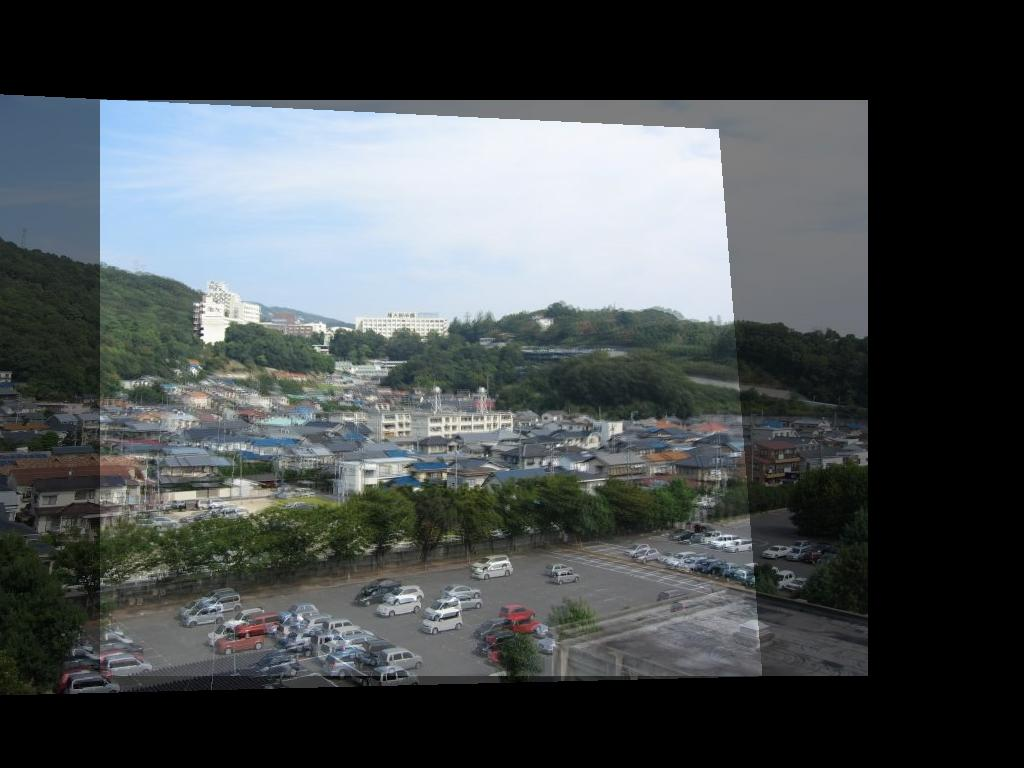
\includegraphics[bb=0 0 1024 768,scale=.2]{../2/panoout.jpg}
\caption{前回の出力画像}
\end{minipage}&
\begin{minipage}{0.5\hsize}
\center
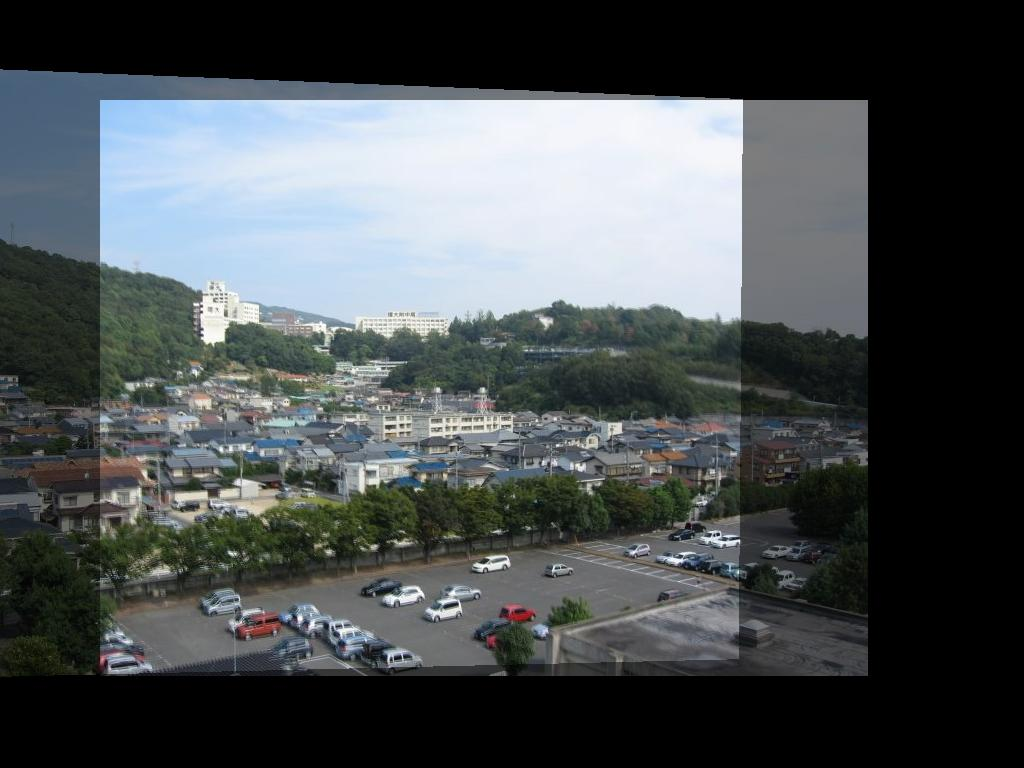
\includegraphics[bb=0 0 1024 768,scale=.2]{out.jpg}
\caption{選んだ対応点から得られた行列を使用した出力画像}
\end{minipage}
\end{tabular}
\end{figure}

前回よりパノラマ画像のクオリティが高くなっている.
これはlsq.cによるものでなく, よりよい対応点の選別によるものであり, 
実際の画像合成アルゴリズムは前回と同様である. 
\end{document}
